\section{Durchführung}
Der Versuchsaufbau besteht aus einer Steckplatine, an die ein Oszilloskop und ein Funktionsgenerator angeschlossen werden können, sowie verschiedenen Elektronikbauteilen. Der exakte Aufbau der einzelnen Versuchsteile wird in \autoref{sec:Schaltungen} beschrieben.

%überall Werte für Widerstände und Kondensatoren ergänzen?

\subsection{Invertierender Linearverstärker}
Es wird ein wie in \autoref{fig:InvLinear} abgebildeter invertierender gegengekoppelter Linearverstärker aufgebaut. Die Ausgangsspannung des Verstärkers wird für drei Verstärkungsgrade, das heißt für drei Widerstandsverhältnisse, in Abhängigkeit der Frequenz gemessen. %(Die Verstärkung fällt mit steigender Frequenz bei sinusförmigen Eingangssignalen ab.) 
Dabei wird ebenfalls die Phase zwischen Ein- und Ausgangssignal gemessen.


\subsection{Umkehr-Integrator}
\label{sec:Umkehr}
Der in \autoref{fig:UmkehrInt} gezeigte Umkehr-Integrator wird aufgebaut.
Es wird die Ein- und Ausgangsspannung in Abhängigkeit der Frequenz gemessen. Das Eingangssignal ist dabei sinusförmig.
%Es wird die Proportionalität zwischen der Ausgangsspannung und dem Kehrwert der Frequenz für ein sinusförmiges Eingangssignal gemessen und so überprüft, dass die gewählte Zeitkonstante sinnvoll ist.

Es werden ein Bildschirmfoto sowie die Daten der Ein- und Ausgangssignale am Oszilloskop für sinusförmige, dreieckförmige und rechteckförmige Eingangssignale gespeichert.



\subsection{Invertierender Differenzierer}
In diesem Versuchsteil wird die Schaltung aus \autoref{fig:InvDiff} aufgebaut und die Schritte aus \autoref{sec:Umkehr} wiederholt.



\subsection{Nicht-invertierende Schmitt-Trigger}
\label{sec:Schmitt}
Die in \autoref{fig:Schmitt} abgebildete Schmitt-Trigger-Schaltung wird aufgebaut und es wird ein sinusförmiges Eingangssignal angelegt. Die Eingangsamplitude wird von ihrem minimal einstellbaren Wert in kleinen Schritten erhöht.
Die Amplitude, bei der die Schaltung beginnt zu kippen, wird bestimmt.
%Alternativ: Dreieckssignal

Am Oszilloskop werden die Daten von Ein- und Ausgangsspannung gespeichert.
%Hysterese-Verlaufskurve ?



\subsection{Signalgenerator}
Hinter die in \autoref{sec:Schmitt} gezeigte Schmitt-Trigger-Schaltung wird ein Integrator gebaut (siehe \autoref{fig:Signal}). Das Eingangssignal ist sinusförmig und das Ausgangssignal dreiecksförmig. Die Frequenz und die Amplitude der erzeugten Schwingung wird bestimmt. 



%\subsection{Variierende Amplituden}
%Die Schaltung für variierende Amplituden wird wie in \autoref{fig:VarAmp} aufgebaut. Der Wert für die Kapazität ist $C = \SI{20}{\nano\farad}$. %oder 100
%Die Dämpfung/ Enddämpfung kann am Potentiometer P zwischen -1 und 1 variiert werden.
%Die \autoref{eq:SchwingAbkling} soll nachgewiesen werden.

%Für den Fall, dass $\eta < 0$ ist, wird eine gedämpfte Schwingung mit dem Oszilloskop aufgenommen. Hier muss zusätzlich eine Rechteckspannung eingespeist werden, da das System nicht von selbst schwingt.

%Für den Fall, dass $\eta > 0$ ist, wird eine charakteristische Frequenz/ Schwingungsdauer ausgemessen.

%\begin{figure}
%    \centering
%    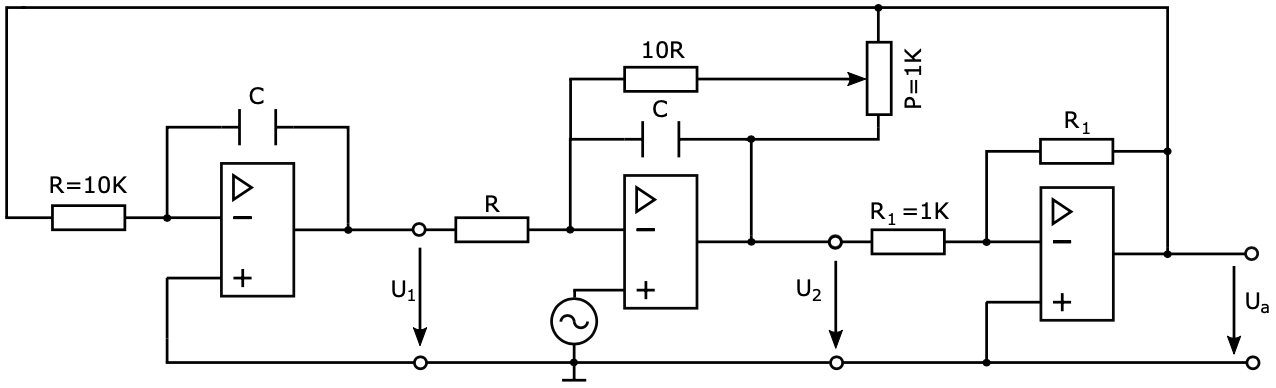
\includegraphics[width=0.7\linewidth]{./figures/6_VarAmp.png}
%    \caption{Aufbau. \cite{Anleitung}}
%    \label{fig:VarAmp}
%\end{figure}